\section{Settings}
\label{section.settings}

The settings screen shows FOQUS settings that are related to the general FOQUS setup, and are unlikely to change between sessions. The settings screen is accessible by clicking the \bu{Settings} button at the top of the Home window. The FOQUS settings can be stored in two locations: (1) ``\%APPDATA\%\bs.foqus.cfg'' on Windows or ``\$HOME/.foqus.cfg'' on Linux or OSX, (2) ``foqus.cfg'' in the working directory.

The Settings screen displays settings grouped into tabs. Figure \ref{fig.settings.options} shows \bu{Settings, FOQUS} tab. 

\begin{figure}[H]
	\begin{center}
		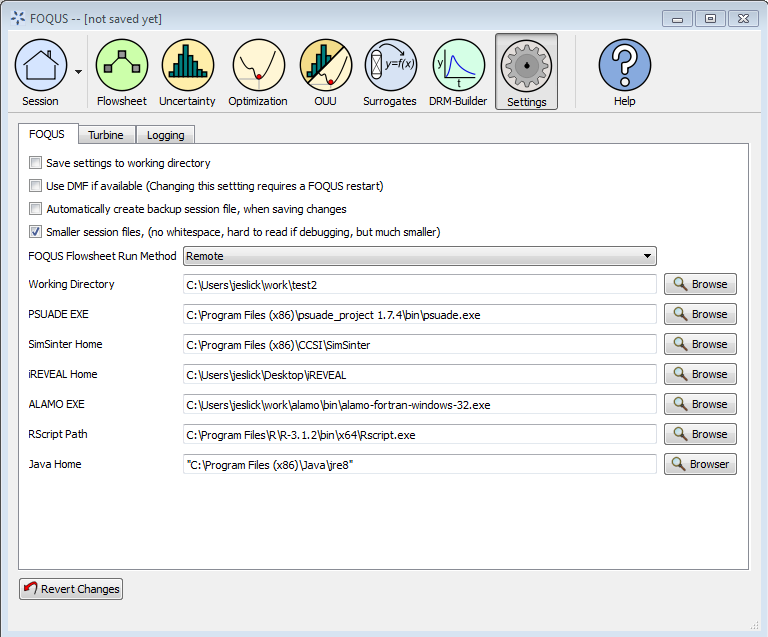
\includegraphics[scale=0.55]{Chapt_flowsheet/figs/settings_options}
		\caption{Settings, FOQUS Tab}
		\label{fig.settings.options}
	\end{center}
\end{figure}

Options in the \bu{Settings, FOQUS} tab are described below.
\begin{enumerate}
	\item  \bu{Save settings to working directoy}, when checkbox is selected the settings file will be read from the specified working directory. This setting is useful for running multiple copies of FOQUS to ensure the settings do not conflict. When starting additional copies of FOQUS, it is best to start them from the Working Directory command line giving each copy of FOQUS its own independent working directory. If FOQUS is started more than once from the Windows start menu, each copy will use the same working directory. Starting FOQUS multiple times with the same working directory may cause unusual behavior in FOQUS.
	\item \bu{Use DMF if available}, when checkbox is selected the Data Management Framework (DMF) module will be loaded and the DMF options will be shown in the \textbf{Session\underline{}} menu.
	\item \bu{Automatically create backup session file}, when checkbox is selected each time a FOQUS session is saved it will be saved twice. A backup copy with a universally unique identifier appended to the file name will be saved.  This will allow the user to load any previous save point of the session.
	\item \bu{Smaller session files}, when checkbox is selected significant storage space is saved by excluding formatting from the session file; this makes the session files less human readable. A more readable session file can be useful for debugging.
	\item \bu{FOQUS Flowsheet Run Method} enables the user to select between running simulations on the same computer as FOQUS, or on a remote Turbine gateway. Running simulations remotely allows parallel execution. The default setting is "Local". If the user switches from "Local" to "Remote", a warning message will appear. The user will be informed that the models that have been uploaded to the Local Turbine may not be available in the Remote Turbine Gateway. Therefore, the user may need to upload these models into Turbine again in order to run the models remotely.
	%Please fix the margins in the paragraph below - Working Directory in the paragraph is displaying beyond the right margin. 
	\item \bu{Working Directory} is the path to the FOQUS working directory. The \textbf{\underline{Working Directory}} is where FOQUS reads and writes files needed to function. When running multiple copies of FOQUS, the \textbf{\underline{Working Directory}} can also be specified from the command line using the ``-w'' or ``--workingDir'' options. After changing the \textbf{\underline{Working Directory}}, FOQUS should be restarted.
	\item \bu{PSUADE EXE} is the path to the PSUADE executable. PSUADE provides FOQUS's UQ features.
	\item \bu{SimSinter Home} is the path to the SimSinter interface for creating Sinter configuration files for simulations to be run with FOQUS. This setting is not required but it allows easy access to the SimSinter configuration GUI when uploading simulation to Turbine.
	\item \bu{iREVEAL Home} is the path the iREVEAL installation. This is required to use the iREVEAL surrogate model module.
	\item \bu{ALAMO EXE} is the path to the ALAMO executable. This is required to use the ALAMO surrogate model module.
	\item \bu{RScript Path} is the path to the RScript executable. This is required for surrogate model modules that use R as a platform.
	\item \bu{Java Home} is the path to the Java installation. The DMF and the iREVEAL surrogate modules require Java.
	\item \bu{Revert Changes} The settings changes are applied when the user navigates away from the settings screen. To undo changes made to settings the revert button can be clicked before changing to another screen.
\end{enumerate}


The \bu{Turbine} tab contains settings for configuring the local and remote instance of Turbine. Figure \ref{fig.settings.turbine} shows the FOQUS Turbine settings.

\begin{figure}[H]
	\begin{center}
		\includegraphics[scale=0.55]{Chapt_flowsheet/figs/settings_turbine}
		\caption{Settings, Turbine Tab}
		\label{fig.settings.turbine}
	\end{center}
\end{figure}

The first section in the \textbf{\underline{Turbine}} tab is \bu{TurbineLite (Local)}. This section contains settings related to the local installation of Turbine, and is only applicable when running FOQUS on the windows platform.
\begin{enumerate}
	\item \bu{Test} tests the connection to the local Turbine server to make sure it is configured and running properly.
	
	\item \bu{Start Service} starts the Turbine server service on Windows. The user must have permission to start services to use this button.
	
	\item \bu{Stop Service} stops the Turbine server service on Windows. The user must have permission to stop services to use this button.
	
	\item \bu{Change Port} can reconfigure the local Turbine server service on Windows to use a different port. This may be necessary if Turbine conflicts with another service.
	
	\item \bu{Aspen Version}, Aspen 7.3 is still in common use but the API differs slightly form newer versions. This option allows FOQUS to be used with Aspen 7.3.
	
	\item \bu{TurbineLite Home} is the location of the TurbineLite installation. For local simulation runs FOQUS needs to know where TurbineLite is installed so it can launch Turbine consumers to run simulations. This setting is not needed if simulations are only run remotely.
		
	\item \bu{Turbine Configuration (local)} is the path to the TurbineLite gateway configuration file for running simulations locally. If simulations are only run remotely, this setting is not needed. \bu{New/Edit} displays a form to create or edit a Turbine configuration file. Having a setting for both local and remote Turbine allows easy switching between run methods.
	
\end{enumerate}

The second section in the \bu{Turbine} tab is \bu{Turbine Gateway (Remote)}. This section contains settings related to a remote instance of Turbine.

\begin{enumerate}
	\item \bu{Test} tests the connection to the remote Turbine server to make sure it is configured and running properly.

	\item \bu{Turbine Configuration (remote)}, is the path to the Turbine gateway configuration file for running simulations remotely. If simulations are only run locally, this setting is not needed. \bu{New/Edit} displays a form to create or edit a Turbine configuration file. Having a setting for both local and remote Turbine allows easy switching between run methods.
	
	\item \bu{Check Interval (sec)} is the number of seconds between checking the remote Turbine server for job results. This number should not be set too low to avoid overwhelming the Turbine server with requests.
	
	\item \bu{Number of Times to Resubmit Failed Jobs} is the number of times to resubmit jobs that fail. Jobs occasionally fail due to software bugs. This allows a job to be retried.

\end{enumerate}

The \bu{Logging} tab contains settings related to the FOQUS log files, which provide debugging information. The FOQUS log files are stored in the logs directory in the working directory. Figure \ref{fig.settings.logging} show the FOQUS log settings. There are two log files (1) FOQUS and (2) Turbine Client.

\begin{figure}[H]
	\begin{center}
		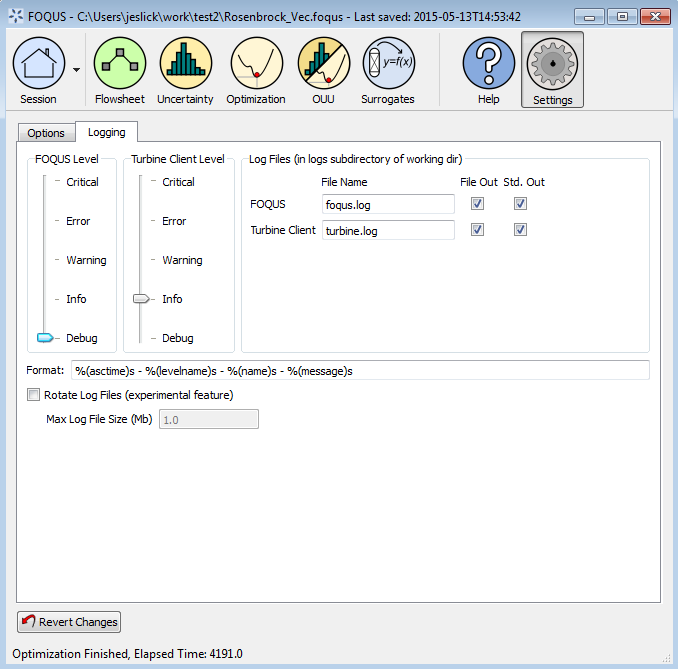
\includegraphics[scale=0.55]{Chapt_flowsheet/figs/settings_logging}
		\caption{Settings, Logging Tab}
		\label{fig.settings.logging}
	\end{center}
\end{figure}

\begin{enumerate}
	\item The level sliders indicate how much information to send to the logs.
	\item The \textbf{\underline{Log Files}} section enables the user to specify where the log information is sent. The \bu{File Out} checkboxes turn on or off the file output of logs. The \bu{Std. Out} checkboxes enable or disable the output to the screen.
	\item \bu{Format} allows the format of the log messages to be changed. See the documentation for the Python 2.7 logging module for more information.
	\item \bu{Rotate Log Files} turns on or off log file rotation. When a log file reaches a certain size, a new log file is started and the contents of the old log are moved to a new file. There currently seems to be a bug in the log file rotation which occasionally makes the log file output stop; therefore, the \bu{Rotate Log Files} option is labeled as an experimental feature.
\end{enumerate}
